\documentclass{article}
\usepackage[utf8]{inputenc}
\usepackage[spanish]{babel}
\usepackage{listings}
\usepackage{graphicx}
\graphicspath{ {images/} }
\usepackage{cite}

\renewcommand{\familydefault}{\sfdefault}

\begin{document}

\begin{titlepage}
    \begin{center}
        \vspace*{1cm}
            
        \Huge
        \textbf{Planteamiento del problema-Pracial 2}
            
        \vspace{0.5cm}
        \LARGE
        
            
        \vspace{5cm}
            
        \textbf{Esteban Felipe Güiza Piñeros}\\
        \textbf{Jose Manuel Rivera Villa }
            
        \vfill
            
        \vspace{0.8cm}
            
        \Large
        Despartamento de Ingeniería Electrónica y Telecomunicaciones\\
        Universidad de Antioquia\\
        Medellín\\
        Septiembre de 2021
            
    \end{center}
\end{titlepage}
\begin{center}
\Huge
\textbf{ANÁLISIS DEL PROBLEMA: }
\end{center}


\subsection{Planteamiento}
La dificultad en el desarrollo de la solución es el impedimento del uso de librerías de redimensionamiento de la imagen, ya que el submuestreo o sobre muestreo de las imágenes debe ser realizado sin la ayuda de estas herramientas, por lo tanto, se debe plantear una alternativa a por medio de un algoritmo que nos permita realizar estas acciones, para seguidamente mostrar esta nueva imagen en TINKERCAD, en el cual se creara un circuito que muestre la imagen redimensionada.

\subsection{}
Después de la implementación del algoritmo, y la elaboración de la estructura en TINKERCAD, debemos complementar toda la estructura y conseguir un proyecto ejecutable y funcional, para eso, el primer paso el planear profundamente la estructura del código. Definir los pasos para el desarrollo del algoritmo, crear las clases y si se requiere añadir contenedores para el desarrollo del código. 

\vspace{12cm}

\begin{center}
\Huge
\textbf{SOLUCION PROPUESTA: }
\end{center}
\subsection{Desarrollo:}
Se planea construir un diagrama que podamos usar para guiar el proceso de desarrollo, y administrar de mejor manera nuestro tiempo. Cada uno de los elementos de este trabajo necesita un gran análisis. La visualización principal de este proyecto se centra en los ejemplos que aparecen en los documentos, para tener una imagen clara de nuestro objetivo y que herramientas utilizar.

\vspace{1cm}

\begin{figure}[h]
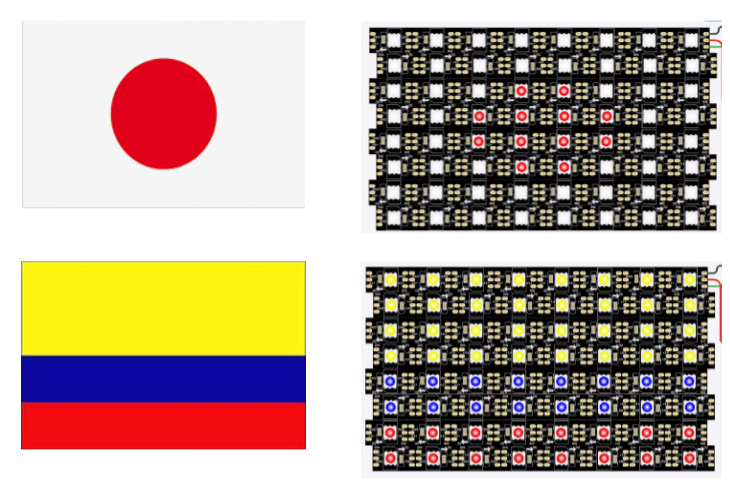
\includegraphics[width=12cm]{image.png}
\centering
\caption{}
\label{fig:tipos}
\end{figure}


\vspace{10cm}
\begin{center}
\Huge
\textbf{ESQUEMA: }
\end{center}

\subsection{Tareas Definidas:}
La idea principal es definir una serie de objetivos a lo largo del periodo de desarrollo que nos permita avanzar en un plazo acorde, y lograr garantizar la estructura del código para que podamos garantizar que todos los componentes funcionen correctamente.




\subsection{Idea inicial}
Para resolver el problema se planteó implementar una clase para poder escalonar una imagen y retornar la matriz correspondiente de colores. en consecuencia, se va a dividir la matriz por una cuadricula del tamaño de la matriz nueva, y en cada sección de la imagen dividida se leen los colores que hay en ese espacio, se suman y se promedian por el total de los pixeles de esa zona, para así tener un promedio del color en ella, se repite este proceso con cada sección de la imagen divida; Con estos datos se crea una nueva matriz la cual será la escalonada de la original. Seguidamente se lleva esta matriz a TINKERCAT, seguidamente solo se leería y se imprimiría en las bandas de leds.


\subsubsection{Esquema  Principal:}
En el Esquema se planean crear diferentes clases, cada una cumplirá diferentes funciones como, la lectura de la imagen que se encargara de almacenarla, el redimensionamiento del tamaño para trabajar con el montaje matricial de leds  10x10  que ya fue implementado en TINKERKAD, y la exportación de la información recopilada de la imagen, que  se incorporara para crear la combinación de colores adecuados para representarla.

1)Se trabajará con Lectura de Imágenes para extraer la información. 
\space{0.5cm}

2)Utilizaremos los contenedores y clases, para desarrollar las primeras bases del código, para extraer la información de la imagen  y almacenarla.
\vspace{0.5cm}

3)Según el procedimiento, se plantea el redimensionamiento de la imagen, que cumpla con las dimensiones ya establecidas en plataforma de TINKERCAD.
\vspace{0.5cm}

4)La salida de este programa será un archivo txt que contendrá el segmento de código que debe ser agregado en el controlador de la matriz de LEDs de la plataforma Arduino.

\vspace{0.5cm}
5)De esta manera al terminar el código y simular, en la matriz de LEDs, se vea representada la imagen indicada por el usuario.
\end{document}


